\documentclass[12pt,a4paper]{report}

% Packages nécessaires
\usepackage[utf8]{inputenc}
\usepackage[T1]{fontenc}
\usepackage[french]{babel}
\usepackage{graphicx}
\usepackage{array}
\usepackage{tabularx}
\usepackage{longtable}
\usepackage{enumerate}
\usepackage{enumitem}
\usepackage{caption}
\usepackage{subcaption}
\usepackage{float}
\usepackage{geometry}
\usepackage{hyperref}
\usepackage{listings}
\usepackage{xcolor}
\usepackage{fancyhdr}
\usepackage{booktabs}
\usepackage{caption}

% Configuration de la géométrie de la page
\geometry{
    a4paper,
    top=2.5cm,
    bottom=2.5cm,
    left=2.5cm,
    right=2.5cm
}

% Configuration des en-têtes et pieds de page
\pagestyle{fancy}
\fancyhf{}
\fancyhead[L]{\leftmark}
\fancyhead[R]{\thepage}

% Configuration des liens hypertexte
\hypersetup{
    colorlinks=true,
    linkcolor=blue,
    filecolor=magenta,      
    urlcolor=cyan,
    pdftitle={Gestion des Résultats d'Analyses Médicales},
    pdfauthor={Votre Nom},
    pdfsubject={Rapport de Projet},
    pdfkeywords={analyses médicales, web, développement}
}

% Configuration des listings de code
\lstset{
    frame=single,
    breaklines=true,
    postbreak=\raisebox{0ex}[0ex][0ex]{\ensuremath{\color{red}\hookrightarrow\space}},
    numbers=left,
    numberstyle=\tiny\color{gray},
    basicstyle=\ttfamily\small,
    keywordstyle=\color{blue},
    stringstyle=\color{green},
    commentstyle=\color{gray},
    showstringspaces=false
}

\begin{document}

% Page de titre
\begin{titlepage}
\begin{center}
    \vspace*{2cm}
    {\Huge\bfseries Gestion des Résultats d'Analyses Médicales\par}
    \vspace{2cm}
    {\Large\itshape Application Web Sécurisée\par}
    \vspace{3cm}
    {\Large Rapport de Projet\par}
    \vspace{3cm}
    {\Large\itshape Réalisé par :\par}
    {\Large Votre Nom\par}
    \vspace{1.5cm}
    {\Large\itshape Encadré par :\par}
    {\Large Nom de l'Encadrant\par}
    \vfill
    {\Large Année Universitaire 2023-2024\par}
\end{center}
\end{titlepage}

% Table des matières
\tableofcontents
\newpage

\chapter{Introduction Générale}

Le domaine de la santé évolue rapidement avec l'intégration des technologies numériques, notamment dans la gestion des données médicales. La gestion des résultats d'analyses médicales est un aspect crucial de ce processus, car ces informations doivent être accessibles rapidement aux patients pour permettre un suivi médical efficace. Cependant, les systèmes traditionnels présentent des limitations : retard dans la transmission des résultats, difficulté d'accès pour les patients, et fragmentation des données médicales à travers différents systèmes.

Ce projet a pour objectif de développer une \textbf{application web} pour la gestion des résultats d'analyses médicales. Cette solution sera spécifiquement orientée vers l'expérience \textbf{patient}, en permettant un accès facile et sécurisé aux résultats. L'application vise à centraliser toutes les informations médicales concernant les analyses effectuées par le patient, lui évitant ainsi les déplacements physiques ou la nécessité de contacter directement les laboratoires.

Le rapport détaille les aspects liés à la conception et au développement de cette application, avec un focus sur la simplicité d'utilisation pour le patient et l'assurance d'une gestion sécurisée de ses résultats médicaux.

\chapter{Cadre Général du Projet}

\section{Introduction}
Le projet vise à améliorer l'accès des patients à leurs résultats d'analyses médicales via une plateforme en ligne simple et sécurisée. L'accès à ces informations est souvent laborieux, avec des systèmes peu intégrés et difficilement accessibles à distance. Ce projet propose une application web qui centralise les résultats d'analyses des patients, avec une interface intuitive qui facilite la consultation des résultats.

\section{Contexte et Problématique}
Actuellement, les patients rencontrent de nombreuses difficultés pour accéder à leurs résultats d'analyses médicales. Les systèmes traditionnels obligent souvent les patients à se déplacer vers les laboratoires ou à passer par des processus compliqués pour récupérer ces informations. De plus, ces systèmes manquent d'intégration, ce qui entraîne une dispersion des résultats et des difficultés à maintenir un historique complet et facilement consultable.

Les patients, dans un monde où l'accès aux services en ligne devient de plus en plus courant, recherchent des solutions leur permettant de consulter leurs résultats sans contrainte de lieu ou de temps. Ce besoin de simplicité, de rapidité et d'accessibilité est au cœur de la solution proposée.

\section{Solution Proposée}
L'application web pour la gestion des résultats d'analyses médicales offrira une solution spécifiquement dédiée aux \textbf{patients}. Les principales fonctionnalités de l'application sont :

\begin{itemize}
    \item \textbf{Création de comptes patients} : Les patients pourront créer un compte sécurisé pour accéder à leurs résultats.
    \item \textbf{Consultation des résultats d'analyses} : Chaque patient aura la possibilité de consulter ses résultats en ligne après leur publication par le laboratoire.
    \item \textbf{Téléchargement des résultats} : Les patients pourront télécharger leurs résultats en format PDF, afin de les conserver ou de les partager facilement avec leurs médecins.
    \item \textbf{Historique des analyses} : L'application permettra aux patients de consulter l'historique complet de leurs analyses médicales, facilitant ainsi le suivi de leur santé.
\end{itemize}

L'application sera simple d'utilisation et ne nécessitera aucune connaissance technique de la part des utilisateurs. Elle mettra en avant la protection et l'accessibilité des informations médicales sans fonctionnalité de notification intégrée, afin de répondre au besoin direct des patients de manière épurée.

\section{Méthodologie de Développement}
Le développement de l'application suivra une méthodologie \textbf{agile}, en adoptant le cadre Scrum pour une approche itérative. Les besoins des patients seront priorisés, avec des retours réguliers pour ajuster et améliorer l'expérience utilisateur.

\subsection{Les rôles au sein de l'équipe Scrum}
\begin{itemize}
    \item \textbf{Product Owner} : Responsable de définir les besoins patients et de prioriser les fonctionnalités qui y répondent.
    \item \textbf{Scrum Master} : Garant du respect du processus agile et de la facilitation des sprints.
    \item \textbf{Équipe de développement} : Composée de développeurs, designers et testeurs, elle sera chargée de la mise en œuvre des fonctionnalités de l'application.
\end{itemize}

\subsection{Organisation des Sprints}
Le projet sera organisé en plusieurs sprints :

\begin{itemize}
    \item \textbf{Sprint 0} : Définition de l'architecture et des besoins fonctionnels de l'application.
    \item \textbf{Sprint 1} : Développement des fonctionnalités de base pour la création et la gestion des comptes patients.
    \item \textbf{Sprint 2} : Implémentation des fonctionnalités de consultation et téléchargement des résultats d'analyses.
    \item \textbf{Sprint 3} : Mise en place de l'historique des analyses, permettant aux patients de consulter l'évolution de leurs résultats au fil du temps.
\end{itemize}

\section{Conclusion}
Ce chapitre a introduit le cadre du projet et les solutions envisagées pour répondre aux problématiques d'accès aux résultats d'analyses médicales par les patients. La solution proposée centralise les informations et simplifie l'accès aux données médicales pour les patients, tout en respectant des normes élevées de sécurité des données.


\chapter{Sprint 0 – Phase de Préparation}

\section{Introduction}
Le Sprint 0 marque la phase de préparation du projet LabConnect. Cette étape est essentielle pour définir les bases du projet, identifier les acteurs et les besoins, et concevoir l'architecture générale avant de commencer le développement. Elle permet également d'établir l'environnement de travail et les technologies à utiliser tout au long du projet.

\section{Modélisation du Contexte et Identification des Acteurs}

\subsection{Identification des Acteurs}
Dans ce projet, nous distinguons plusieurs acteurs clés :

\begin{itemize}
    \item \textbf{Utilisateur} : Il s'agit des patients qui se connectent pour accéder à leurs résultats d'analyses médicales.
    
    \item \textbf{Administrateur du Laboratoire} : Responsable de l'ajout et de la gestion des résultats sur la plateforme.
    
    \item \textbf{Système} : Le serveur backend qui gère les données, l'authentification, et la sécurité des échanges entre les utilisateurs et les laboratoires.
\end{itemize}

\subsection{Diagramme de Cas d'Utilisation}
\begin{figure}[h]
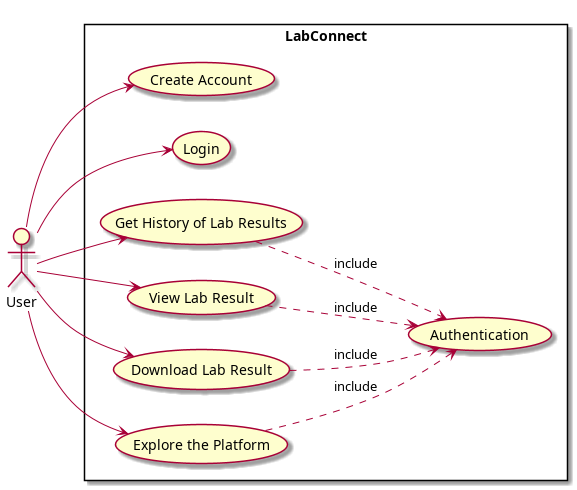
\includegraphics[width=\textwidth]{./img/diagram/UseCases/global.png}
\caption{Diagramme de cas d'utilisation du système LabConnect}
\label{fig:use-case}
\end{figure}

\section{Spécification des Besoins}

\subsection{Besoins Fonctionnels}
Les besoins fonctionnels identifiés pour le projet LabConnect incluent :

\begin{itemize}
    \item Création et gestion des comptes utilisateurs (inscription, connexion, modification des informations).
    \item Consultation et téléchargement des résultats d'analyses médicales.
    \item Gestion des données utilisateurs par les administrateurs des laboratoires.
    \item Sécurisation des données médicales à travers un système d'authentification robuste.
\end{itemize}

\subsection{Besoins Non Fonctionnels}
En plus des besoins fonctionnels, plusieurs besoins non fonctionnels ont été identifiés :

\begin{itemize}
    \item \textbf{Sécurité} : Protection des données médicales des utilisateurs à travers l'authentification et le chiffrement des données.
    \item \textbf{Performance} : Rapidité dans la récupération des résultats et fluidité de l'expérience utilisateur.
    \item \textbf{Scalabilité} : Capacité à gérer un nombre croissant d'utilisateurs et de données.
\end{itemize}

\section{Analyse Globale}

\subsection{Architecture Logique}
\begin{figure}[h]
    \centering
    % [Placeholder pour le schéma d'architecture logique]
    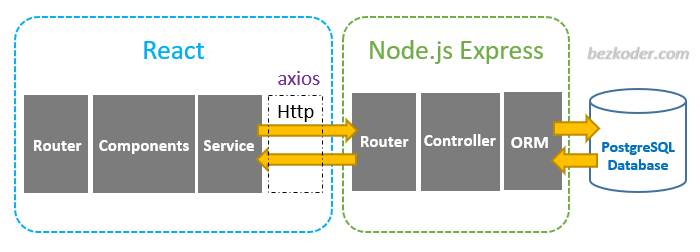
\includegraphics[width=\textwidth]{./img/ph/ph.png}
    \caption{Architecture logique de LabConnect}
    \label{fig:logical-architecture}
\end{figure}

\section{Pilotage du Projet avec Scrum}

\subsection{Backlog Produit}
Le backlog produit comprend l'ensemble des fonctionnalités à développer pour LabConnect. Il est divisé en plusieurs catégories :

\begin{itemize}
    \item \textbf{Interface utilisateur} (landing page, gestion des comptes)
    \item \textbf{Système d'authentification} (inscription, connexion, récupération de mot de passe)
    \item \textbf{Gestion des résultats médicaux} (lecture, téléchargement, stockage sécurisé)
\end{itemize}

\subsection{Planification des Sprints}
Le projet sera divisé en plusieurs sprints :

\begin{enumerate}
    \item \textbf{Sprint 1} : Conception de la base de données, des routes et de l'API, et développement de la landing page.
    \item \textbf{Sprint 2} : Implémentation des fonctionnalités d'authentification et du front-end associé.
    \item \textbf{Sprint 3} : Gestion des résultats médicaux et développement des interfaces pour leur consultation.
\end{enumerate}

\section{Environnement de Travail}

\subsection{Environnement Logiciel}
L'environnement logiciel choisi pour le développement de LabConnect inclut :

\begin{itemize}
    \item \textbf{Backend} : Node.js avec Express pour la création de l'API.
    \item \textbf{Base de données} : MongoDB pour la gestion des données utilisateurs et des résultats médicaux.
    \item \textbf{Frontend} : HTML, CSS, et JavaScript pour le développement de l'interface utilisateur.
\end{itemize}

\subsection{Technologies Utilisées}
\begin{itemize}
    \item \textbf{Frameworks et Librairies} : Utilisation d'Express.js pour la gestion des routes, de Mongoose pour interagir avec la base de données MongoDB, et de Bootstrap pour la mise en page front-end.
    \item \textbf{Système d'authentification} : Utilisation de JWT (JSON Web Tokens) pour sécuriser l'authentification des utilisateurs.
\end{itemize}

\section{Conclusion}
Le Sprint 0 constitue une étape clé dans la préparation du projet LabConnect. Il permet d'identifier les besoins fonctionnels et non fonctionnels, de définir les acteurs, et de concevoir l'architecture globale du système. Avec un environnement de travail bien établi et une méthodologie Scrum pour piloter le projet, l'équipe est prête à passer à la phase de développement.
\chapter{Étude et réalisation du Sprint 1}

\section{Introduction}

Le Sprint 1 de LabConnect est dédié à la mise en place de la base de données, des routes, et de l’API, ainsi que le développement de la page d'accueil (\textit{landing page}). Ce sprint vise à fournir les bases techniques nécessaires pour supporter les fonctionnalités d'authentification et de gestion des résultats médicaux dans les sprints suivants.

\section{Backlog du Sprint 1}

Le backlog du Sprint 1 est axé sur les tâches suivantes :

\begin{itemize}
    \item Conception de la base de données.
    \item Création des routes et API pour la communication entre le front-end et le back-end.
    \item Développement de la \textit{landing page} pour présenter le service.
    \item Mise en place d’une structure de projet permettant la scalabilité.
\end{itemize}

\section{Analyse et spécification des besoins}

\subsection{Diagramme de cas d’utilisation global du Sprint 1}

\textbf{[Insérer ici un diagramme de cas d’utilisation montrant les interactions des utilisateurs avec les composants développés lors du Sprint 1]}

\subsection{Description textuelle de cas d’utilisation}

\textbf{Cas d’utilisation 1 :}

\begin{itemize}
    \item \textbf{Titre :} Visualisation de la page d'accueil.
    \item \textbf{Acteur principal :} Utilisateur non authentifié.
    \item \textbf{Description :} L’utilisateur accède à la \textit{landing page} pour consulter les services offerts par LabConnect. Aucun compte n'est requis pour cette action.
    \item \textbf{Scénario :}
    \begin{enumerate}
        \item L'utilisateur ouvre le navigateur et entre l'URL de LabConnect.
        \item Le serveur renvoie la \textit{landing page}.
        \item L'utilisateur parcourt les informations disponibles sur la page.
    \end{enumerate}
\end{itemize}

\textbf{Cas d’utilisation 2 :}

\begin{itemize}
    \item \textbf{Titre :} Accès aux routes API.
    \item \textbf{Acteur principal :} Système.
    \item \textbf{Description :} Le système reçoit des requêtes API pour différentes actions telles que la création de comptes ou la récupération de données.
    \item \textbf{Scénario :}
    \begin{enumerate}
        \item Le client envoie une requête API (par exemple, pour récupérer des informations utilisateur).
        \item Le serveur traite la requête via les routes définies et renvoie une réponse appropriée.
    \end{enumerate}
\end{itemize}

\section{Services Web}

Les services web sont assurés via une API RESTful développée avec Node.js et Express. Les principales routes créées dans ce sprint sont les suivantes :

\begin{itemize}
    \item \textbf{GET / :} Route pour afficher la \textit{landing page}.
    \item \textbf{API /api/users :} Route pour la gestion des utilisateurs.
    \item \textbf{API /api/results :} Route pour gérer l'accès aux résultats d'analyses (créée mais non encore fonctionnelle dans ce sprint).
\end{itemize}

L’API est conçue pour être extensible et s’adapter aux fonctionnalités futures, notamment pour gérer les authentifications et les résultats des laboratoires.

\section{Réalisation (pour les interfaces graphiques)}

Au cours de ce sprint, une attention particulière a été portée à l’interface utilisateur de la \textit{landing page} :

\begin{itemize}
    \item \textbf{Technologies utilisées :} HTML, CSS, et Bootstrap pour une mise en page \textit{responsive} et conviviale.
    \item \textbf{Contenu de la page :} Présentation des services proposés par LabConnect, section contact, et informations de base sur la sécurité des données médicales.
\end{itemize}

\textbf{[Insérer ici des captures d’écran de l’interface développée si nécessaire]}

\section{Conclusion}

Le Sprint 1 constitue la fondation du projet LabConnect. Il assure la structure nécessaire au développement des fonctionnalités à venir. Grâce à une API flexible et une \textit{landing page} attrayante, le projet est prêt à évoluer vers l’intégration des systèmes d’authentification et de gestion des résultats dans les prochains sprints.

\chapter{Étude et réalisation du Sprint 2}

\section{Introduction}

Le Sprint 2 de LabConnect se concentre sur la mise en place de la fonctionnalité d'authentification. Ce sprint inclut l'inscription des utilisateurs, la connexion, et la gestion de l'accès aux services de la plateforme. L'objectif est de permettre aux utilisateurs de créer un compte sécurisé, de se connecter à la plateforme et d'accéder à leurs données personnelles et résultats d'analyses médicales.

\section{Backlog du Sprint 2}

Le backlog de ce sprint comprend les tâches suivantes :

\begin{itemize}
    \item Mise en place du système d'inscription et de connexion.
    \item Création des routes et de l’API associées pour l’authentification.
    \item Développement de l’interface utilisateur pour les formulaires d’inscription et de connexion.
    \item Gestion des erreurs et validation des données d’authentification.
\end{itemize}

\section{Analyse et spécification des besoins}

\subsection{Diagramme de cas d’utilisation global du Sprint 2}

\textbf{[Insérer ici un diagramme de cas d’utilisation montrant les interactions des utilisateurs avec le système d’authentification développé pendant le Sprint 2]}

\subsection{Description textuelle de cas d’utilisation}

\textbf{Cas d’utilisation 1 :}

\begin{itemize}
    \item \textbf{Titre :} Inscription d’un nouvel utilisateur.
    \item \textbf{Acteur principal :} Utilisateur non authentifié.
    \item \textbf{Description :} Un utilisateur s'inscrit sur la plateforme en remplissant un formulaire avec ses informations personnelles.
    \item \textbf{Scénario :}
    \begin{enumerate}
        \item L'utilisateur accède à la page d'inscription.
        \item Il remplit les champs requis (nom, email, mot de passe).
        \item Le système valide les données et crée un nouveau compte.
        \item Un message de confirmation est affiché à l'utilisateur.
    \end{enumerate}
\end{itemize}

\textbf{Cas d’utilisation 2 :}

\begin{itemize}
    \item \textbf{Titre :} Connexion à un compte existant.
    \item \textbf{Acteur principal :} Utilisateur authentifié.
    \item \textbf{Description :} Un utilisateur déjà inscrit peut se connecter à son compte en fournissant ses identifiants.
    \item \textbf{Scénario :}
    \begin{enumerate}
        \item L'utilisateur accède à la page de connexion.
        \item Il entre son email et son mot de passe.
        \item Le système valide les informations et l'utilisateur est redirigé vers son tableau de bord personnel.
    \end{enumerate}
\end{itemize}

\section{Conception}

\subsection{Diagramme de séquence du Sprint 2}

\textbf{[Insérer ici un diagramme de séquence détaillant le processus d'inscription et de connexion, montrant l'interaction entre le client, le serveur, et la base de données]}

\section{Services Web}

Dans ce sprint, l'API est enrichie avec les services d'authentification. Les routes suivantes ont été ajoutées :

\begin{itemize}
    \item \textbf{POST /api/register :} Permet l'inscription d'un nouvel utilisateur.
    \item \textbf{POST /api/login :} Permet la connexion d'un utilisateur existant.
    \item \textbf{GET /api/logout :} Permet la déconnexion d’un utilisateur.
\end{itemize}

L'API gère également la validation des données utilisateur (par exemple, format de l'email, sécurité du mot de passe).

\section{Réalisation (pour les interfaces graphiques)}

Pour les interfaces graphiques, les pages suivantes ont été développées :

\begin{itemize}
    \item \textbf{Page d'inscription :} Formulaire permettant à l'utilisateur de s'inscrire.
    \item \textbf{Page de connexion :} Formulaire permettant à l'utilisateur de se connecter.
\end{itemize}

Technologies utilisées : HTML, CSS, et JavaScript. Des bibliothèques comme Bootstrap ont été employées pour garantir une expérience utilisateur fluide et responsive.

\section{Test}

Pendant ce sprint, des tests ont été effectués pour valider le bon fonctionnement du système d'authentification. Les scénarios suivants ont été testés :

\begin{itemize}
    \item Inscription avec des données valides.
    \item Inscription avec des données invalides (par exemple, email incorrect, mot de passe trop court).
    \item Connexion avec des identifiants valides.
    \item Connexion avec des identifiants incorrects.
    \item Déconnexion.
\end{itemize}

Outils utilisés pour les tests : Postman pour les tests d'API et des outils de test manuels pour l'interface utilisateur.

\section{Conclusion}

Le Sprint 2 a permis de mettre en place l’authentification des utilisateurs, une composante essentielle du projet LabConnect. Grâce à une API robuste et une interface utilisateur intuitive, les utilisateurs peuvent désormais créer un compte et accéder à leurs données. Ce sprint fournit également une base solide pour l’intégration des résultats médicaux dans le sprint suivant.
\chapter{Étude et réalisation du Sprint 3}

\section{Introduction}

Le Sprint 3 de LabConnect est consacré à l'intégration des fonctionnalités de gestion des résultats médicaux. Les utilisateurs authentifiés pourront désormais consulter et télécharger leurs résultats d'analyses. Ce sprint met l'accent sur la gestion sécurisée des données médicales, la présentation des résultats dans une interface utilisateur claire, et la possibilité de télécharger les fichiers de manière sécurisée.

\section{Backlog du Sprint 3}

Les tâches incluses dans le backlog de ce sprint sont les suivantes :

\begin{itemize}
    \item Développement des routes et API pour la gestion des résultats médicaux.
    \item Création de l'interface utilisateur pour afficher les résultats d'analyses.
    \item Mise en place de la fonctionnalité de téléchargement des résultats.
    \item Assurer la sécurité et la confidentialité des données médicales.
\end{itemize}

\section{Analyse et spécification des besoins}

\subsection{Diagramme de cas d’utilisation global du Sprint 3}

\textbf{[Insérer ici un diagramme de cas d’utilisation montrant les interactions entre les utilisateurs et le système pour la gestion des résultats médicaux]}

\subsection{Description textuelle de cas d’utilisation}

\textbf{Cas d’utilisation 1 :}

\begin{itemize}
    \item \textbf{Titre :} Visualisation des résultats médicaux.
    \item \textbf{Acteur principal :} Utilisateur authentifié.
    \item \textbf{Description :} L'utilisateur accède à son espace personnel pour consulter la liste de ses résultats médicaux.
    \item \textbf{Scénario :}
    \begin{enumerate}
        \item L'utilisateur se connecte à la plateforme.
        \item Il accède à la section "Résultats médicaux".
        \item La liste de ses analyses médicales lui est présentée.
        \item L'utilisateur sélectionne un résultat pour le consulter en détail.
    \end{enumerate}
\end{itemize}

---

\textbf{Cas d’utilisation 2 :}

\begin{itemize}
    \item \textbf{Titre :} Téléchargement des résultats médicaux.
    \item \textbf{Acteur principal :} Utilisateur authentifié.
    \item \textbf{Description :} L'utilisateur télécharge un fichier PDF contenant les détails de ses analyses médicales.
    \item \textbf{Scénario :}
    \begin{enumerate}
        \item L'utilisateur accède à son espace personnel.
        \item Il sélectionne un résultat médical dans la liste.
        \item Il clique sur le bouton "Télécharger" pour obtenir une copie du résultat sous forme de fichier PDF.
        \item Le fichier est téléchargé sur son appareil.
    \end{enumerate}
\end{itemize}

\section{Conception}

\subsection{Diagramme de séquence du Sprint 3}

\textbf{[Insérer ici un diagramme de séquence décrivant l'interaction entre le client, le serveur, et la base de données pour la récupération et le téléchargement des résultats médicaux]}

\section{Réalisation (pour les interfaces graphiques)}

L'interface utilisateur du Sprint 3 comprend les pages suivantes :

\begin{itemize}
    \item \textbf{Page de résultats médicaux :} Présente la liste des résultats d'analyses de l'utilisateur, avec la possibilité de consulter et de télécharger chaque résultat.
    \item \textbf{Interface de téléchargement :} Intègre un bouton permettant de télécharger les résultats médicaux sous forme de PDF.
\end{itemize}

Technologies utilisées : HTML, CSS, JavaScript, et Bootstrap pour une interface responsive et conviviale. L'affichage des résultats est optimisé pour la clarté et la facilité de navigation.

\section{Test}

Divers scénarios ont été testés pour garantir le bon fonctionnement des fonctionnalités de gestion des résultats médicaux :

\begin{itemize}
    \item Consultation de la liste des résultats médicaux.
    \item Vérification de l'affichage correct des informations.
    \item Téléchargement des fichiers PDF et validation de l’intégrité des fichiers téléchargés.
    \item Tests de sécurité pour s'assurer que seuls les utilisateurs authentifiés peuvent accéder à leurs propres résultats.
\end{itemize}

Outils utilisés pour les tests : Postman pour les tests d’API, et des tests manuels ont été réalisés pour valider l'interface utilisateur.

\section{Conclusion}

Le Sprint 3 marque une étape cruciale dans le projet LabConnect avec l'intégration de la fonctionnalité clé : la gestion des résultats médicaux. Les utilisateurs peuvent désormais consulter et télécharger leurs analyses médicales de manière sécurisée. Ce sprint pose les bases pour d'éventuelles extensions futures, comme la visualisation graphique des résultats ou la notification des nouveaux résultats disponibles.


% Bibliographie
\begin{thebibliography}{9}
\bibitem{ref1} Auteur1, \textit{Titre1}, Éditeur, Année.
\bibitem{ref2} Auteur2, \textit{Titre2}, Éditeur, Année.
\end{thebibliography}

\end{document}